	Here we present some results from stochastic analysis. This chapter focus on
provide the basic information and tools to understand the nature of a SDE and its numerical approximation. For reference
see \cite{Arnold1979, Kloeden1992, Williams1991, Milstein2004, Resnick2003}.

\section{Probability theory and Stochastic Processes}
		Probability theory  is the field that  studies the random phenomena. A random event is the set of  outcomes from an 
experiment conducted under the same conditions  with a variability in results . Probability theory aims to 
describe  this variability. We denote by $\Omega$ the set of observable outcomes, $\omega$, from a
experiment or phenomenon.  However, not every observable event is measurable, so  for the purpose of probability 
theory, a family of subsets from $\Omega$ with particular properties  a ----$\sigma$-algebra is needed. In 
the following, we formalize these concepts.	


\begin{definition}[$\sigma$-algebra]
	Let $\Omega$ a set and $\calF$ a family of subset of $\Omega$, we call $\calF$ a 
	$\sigma$- algebra if the following properties hold:
	\begin{enumerate}[(i)]
		\item $\emptyset \in \calF$,
		\item if $F\in \calF$ then $F^c\in\calF$ where $F^c = \Omega \setminus F$,
		\item if $\displaystyle \{F_i\}_{i=1}^\infty \in \calF $ then 
			$\displaystyle \bigcup_{i\geq 1} F_i \in \calF$.
	\end{enumerate}
\end{definition}

	Let $\calC$ a collection of subsets of $\Omega$. The $\sigma$-algebra generated by $\calC$
denoted by $\sigma(\calC)$, is the smallest $\sigma$-algebra which contains the collection $\calC$, that is
$\sigma(\calC)\supset \calC$, and if $\calB$ is an other $\sigma$-algebra containing $\calC$, then
$\calB \supset \sigma(\calC)$.
\begin{definition}[The Borel $\sigma$-algebra]
	The $\sigma$-algebra generated by the collection of all open sets $U \subset \Omega$ 
\end{definition}
	
	A probability space is a triple $(\Omega, \calF, \P)$ where
\begin{itemize}
	\item $\Omega$ is the set of all possible outcomes of an experiment.
	\item $\calF$ is a conveniently $\sigma$-algebra of subsets of $\Omega$.
	\item $\P$ is a probability measure; that is a function $\P: \calF \to [0,1]$ such that
	\begin{enumerate}[(i)]
		\item
			$\P(A)\geq 0$ for all $A \in \calF$.
		\item
			$\P$ is $\sigma$-additive, that is: If $\{A_n,  n\geq 1 \}$ is a collection of disjoint events,
			then
				$$
					\P \left(
						\bigcup_{n=1}^{\infty} A_n
					\right)= \sum_{n=1}^{\infty}
						\P(A_n).
				$$
		\item
			$\P(\Omega) = 1$.
	\end{enumerate}
\end{itemize}
\begin{definition}[Random Variable]
	Let $(\Omega, \calF, \P)$ be a probability space and $\calB(\R^d)$ the Borel's $\sigma$-algebra. A  function $X:\Omega \to \R^n$ is said to be a random variable if $X$ is $(\calF,\calB(\R^d))$-measurable, that is
	$
		X^{-1}(\calB(\R^d))\subset \calF
	$.
\end{definition}
	Every random variable $X$ induces a probability measure $\mu_X$ on $\R^d$ by
	$$
		\mu_{X}(B) = \P(X^{-1}(B)), \qquad B\in\calB(\R^d).
	$$ 
%

	Having two different measures $\Q$, $\P$, on a measurable space we can transform one measure into the
other via  Radon-Nikodym theorem  (see for example \cite[Thm. 10.1.2]{Williams1991}).

\begin{thm}[Radon-Nikodym]
	Let $\P$ and $\Q$ probability measures on the measurable space $(\Omega,\calF)$. Suppose that for all
	$B\in\calF$ $\Q(B)=0$ implies $\P(B)=0$. Then there exist a integrable random variable $X$ such that
	$$
		\Q(E) = \int_{E}Xd\P, \qquad \forall E\in\calF.
	$$
	$X$ is $\P$-a.s. unique and is written as $\displaystyle X = \frac{d\Q}{d\P}$.
\end{thm}
	This important result describes the density $p$ of a random variable $X$ as the $\P$-a.s.
unique Radon-Nikodym derivative of the induced distribution $\mu_{X}$ w.r.t. Lebesgue measure, in other 
words
$$
	\mu_{X}(B)=\int_{B} p(x)dx.
$$

\begin{definition}[Expectation]
	Let $X$ be a integrable random variable on a probability space $(\Omega, \calF, \P)$. Then the expectation
	of $X$ is defined by
	\begin{equation*}
		\EX{X}= \int_{\Omega} X(\omega) \P(d\omega).
	\end{equation*}
\end{definition}

		
	A stochastic process $X$ is a system which could stay at each moment on any state of a given set $S$
\begin{definition}[Stochastic Process]
	A stochastic process is a collection of random variables $X=\{X_t: t \in T\}$ on $(\Omega,
	\calF)$,  which takes values in a measurable space $(S,\calS)$, and where the index $t\in [0,\infty)$, 
	conveniently receive an interpretation as time. Thus for a fixed $\omega \in \Omega$, the function
	$X_t(\omega)$, $t\geq 0$ is a sample path of the process $X$ associated with $\omega$,  and for any
	fixed $t$ , $X_t(\omega)$, $\omega \in \Omega$ is a random variable. 

\end{definition}
 The main purpose of this thesis deals with the numerical approximation of sample paths.
\begin{definition}[Measurable Process]
	A stochastic process $X$ is measurable if the mapping
	\begin{equation*}
		(t, \omega) \to X_t(\omega):
		\left(
			[0,\infty)\times \Omega,
			\calB \left(
				[0,\infty)
			\right) \otimes \calF
		\right)
		\to 
		\left(
			\R^d, \calB \left (\R^d \right)
		\right)
	\end{equation*}
	is measurable.
\end{definition}
%
	We equip the underlying sample space $(\Omega, \calF)$ with a filtration $\{\calF\}_{t\geq 0}$ in order to 
keep track information about the past, present and future of a stochastic process. Formally, a filtration is
a nondecreasing family of sub-$\sigma$-algebras of $\calF$ such that 
$\calF_s\subseteq \calF_t \subseteq \calF$ for $0\leq s \leq t <\infty$ and is called right continuous if
$ %\displaystyle
	\calF_t = \bigcap_{r>t} \calF_r
$
for all $t\geq 0$. Thus if the underlying probability space is complete,
right continuous and $\calF_0$ contains all $\P$-null sets, then we say that the filtration
$\{ \calF_t\}_{t\geq 0}$ satisfies the usual conditions. In the following, we will work only on a
complete probability space $(\Omega, \calF, \P)$  with a filtration $\{\calF_t \}_{t \geq 0}$ which verifies
the usual conditions.
	
	Given a stochastic process, the simplest choice of a filtration is that generated
by the process itself, i.e. 
$
	\calF^{X}_t:=\sigma(X_s; 0\leq s\leq t)
$
the smallest $\sigma$-algebra with respect to which $X_s$ is measurable for every $s\in[0, t]$.
The introduction of this concept gives sense to the following.
\begin{definition}[Adapted Process]
		We call a process \it{adapted} to the filtration $\{\calF\}_{t\geq 0}$  if, for each $t>0$ fixed $X_t$  is a
	$\calF_t$-measurable random variable.
\end{definition}
Clearly, every process $X$ is adapted to $\{ \calF_t^{X}\}$.
\begin{definition}[Progressively Measurable Process]
	The stochastic process $X$ is progressively measurable if the mapping
	$$
		(s,\omega)\to X_s(\omega):
		\left(
			[0,t] \times \Omega,
			\calB([0,t]) \otimes \calF_t
		\right) \to 
		\left(
			\R, \calB\left(\R^d\right)
		\right)
	$$
	is measurable for each $t\geq 0$, that is, if, for each $t>0$ and $A\in \calB\left(\R^d\right)$, 
	the set 
	$$
		\{
			(\omega, s) : 0 \leq s \leq t, \omega \in \Omega, X_s(\omega) \in A
		\}
	$$
	belongs to the product $\sigma$-algebra
	$
		\calB([0,t]) \otimes \calF_t
	$.
\end{definition}
%
\subsection{Stopping time}
	\todo{Write an Introduction Paragraph}

\begin{definition}[Stopping Time]
	A random variable $\tau:\Omega \to [0, \infty]$ is called an $\{\calF_{t}\}$-stopping time if
	$\{\omega: \tau(\omega)\leq t \}\in \calF_t$ for any $t\geq 0$.
\end{definition}
%
\begin{thm}
	If $\{ X_t\}_{t\geq 0}$ is a progressively measurable process and $\tau$ is a stopping time,
	then $X_t \1{\tau <\infty}$ is $\{\calF_t \}$-measurable.
\end{thm}
%
\begin{thm}
	Let $\{X_t \}_{t\geq 0}$ be and $\R^d$-valued cádlág $\{\calF_t\}$-adapted process and $D\subset \R^d$ an open set. 
	Then
	$
		\tau := \inf\left\{t \geq 0: X_t \notin D \right\}
	$
	is an $\{\calF_t\}$-stopping time.
\end{thm}
%
\begin{lem}[Fatou]
	For any non negative measurable functions $\{ X_k\}_{k\geq 1}$ on $(\Omega, \calF, \P)$, we have
	$$
	\EX{
		\liminf_{k\to\infty}
		X_k
	} \leq \liminf_{k\to\infty}\EX{X_k}.
	$$
\end{lem}

		\subsection{Conditional Expectation}
		
	Conditional expectation plays a very important role in the modern probability theory. It gives  
foundation for the definitions of martingales and Markov processes. In fact, other areas of probability 
as stochastic dynamics, conditioning permits to describe and to analyze dynamical systems with randomness.
Roughly speaking, the conditional expectation is an average that considers only a portion of information.
Assume $X\in L_1(\Omega,\calF,\P)$ and let $\calG \subset \calF$ a sub-$\sigma$-algebra. Then the
conditional expectation of the random variable $X$ given $\calG$ is the new random variable 
$Y = \cEX{X}{\calG}$ such that
\begin{enumerate}[(i)]
	\item
		$\cEX{X}{G}$ is $\calG$-measurable and integrable.
	\item
		For all event $G\in \calG$ we have 
		$
			\displaystyle
			\int_{G} X d\P = \int_{G} \cEX{X}{\calG}d\P.
		$
\end{enumerate}
	This new random variable is unique in the sense that if there is an other $\tilde{Y}$ satisfying
the same two above properties, then $\P{[Y\neq \tilde{Y}]}=0$. In this case $\tilde{Y}$ is said to be 
a version of the conditional expectation $\cEX{X}{\calG}$.
Now we list some standard properties of the conditional expectation \cite{Williams1991}.
Here $X_1$, $X_2$, $Z$ are integrable random variables, $a_1$,$a_2\in \R$, and $\calG$, $\calH$ 
are sub-$\sigma$-algebras of $\calF$.
\begin{enumerate}[(E1)]
	\item
		If $Y$ is any version of $\cEX{X}{\calG}$, then $E[X]=E[Y]$.
	\item
		If $X$ is $\calG$ measurable, then $\cEX{X}{\calG} = X$, $\P$-a.s.
	\item
		(Linearity) $\cEX{a_1X_1+a_2X_2}{\calG} = a_1\cEX{X_1}{\calG} + a_2\cEX{X_2}{\calG}$ $\P$-a.s.\\
		Clarification:
			if $Y_1$ is a version of $\cEX{X_1}{\calG}$ and $Y_2$ is a version of $\cEX{X_2}{\calG}$, then
			$a_1Y_1 + a_2Y2$ is a version of $\cEX{a_1 X_1 + a_2X_2}{\calG}$.
	\item
		(Positivity) If $X \geq 0$, then $\cEX{X}{\calG} \geq 0$,  $\P$-a.s.
	\item
		(Conditional Monotone Convergence)
		If $0 \leq X_n \uparrow X$, then $\cEX{X_n}{\calG} \uparrow \cEX{X}{\calG}$, $\P$-a.s.
	\item
		(Conditional Fatou)
		If $X_n\geq 0$, then 
		$\displaystyle
			\cEX{\liminf_{n \to \infty} X_n}{\calG}
			\leq
			\liminf_{n \to \infty}
			\cEX{X_n}{\calG}
		$.
	\item
		(Conditional Dominated Convergence)
		If $|X_n(\omega)|\leq V(\omega)$ for all $n$, $\EX{V}<\infty$, and $X_n \to X$ $\P$-a.s., then
		$\cEX{X_n}{\calG} \to \cEX{X}{\calG}$, $\P$-a.s.
	\item
		(Conditional Jensen)
		If $f$ is a real-valued convex function, then
		$$
			f
			\left(
				\cEX{X}{\calG}
			\right)
			\leq
			\cEX{f(X)}{\calG}.
		$$
		\item
			(Tower Property) If $\calH$ is a sub-$\sigma$-algebra of $\calG$, then
			$$
				\cEX{\cEX{X}{\calG}}{\calH} = \cEX{X}{\calH}, \qquad \P\text{-a.s.}.
			$$
		\item
			If $Z$ is $\calG$-measurable and bounded, then
			$
				\cEX{ZX}{\calG} = Z\cEX{X}{\calG}.
			$
		\item
			If $X$ is independent from $\calH$, then
			$\cEX{X}{\calH} = \EX{X}$, \qquad $\P$-a.s.
\end{enumerate}

	Now consider a filtered space $\left(\Omega, \calF, \{\calF_t\}_{t\geq 0}, \P \right)$ and define
$$
	\calF_{\infty}:= \sigma
		\left(
			\bigcup_{t\geq 0}
			\calF_t
		\right) \subset \calF.
$$

\begin{definition}[Martingale]
	A process $\{M_t\}_{t\geq 0}$ is called a martingale (relative to $\left(\{F_t \}_{t\geq 0}, \P \right)$ if
	\begin{enumerate}[(i)]
		\item
			$M$ is adapted,
		\item
			$\EX{|M_t|}<\infty$ \qquad for all $t\geq 0$,
		\item\label{dfn:Martingale}
			$
				\cEX{M_t}{\calF_s} = M_s
			$, \qquad $\P$-a.s., \qquad $0\leq s \leq t$.
	\end{enumerate}
\end{definition}

	In this way, a \emph{supermartingale} (relative to $\left(\{F_t \}_{t\geq 0}, \P \right)$ is defined similarly, 
except that \eqref{dfn:Martingale} is replaced by
$$
	\cEX{M_t}{\calF_s}\leq M_s
	\qquad \P\text{-a.s.},
	\qquad 0\leq s \leq t, 
$$ and a \emph{submartingale} is defined with \eqref{dfn:Martingale} 
replaced by
$$
	\cEX{M_t}{\calF_s} \leq M_s
	\qquad \P\text{-a.s.},
	\qquad 0\leq s \leq t.
$$ 
\begin{thm}
	Let $\{M_t\}_{t\geq 0}$ be and $\R^d$-valued martingale with respect to $\{\calF_t\}$, and let $\theta$, $\rho$ two 
	finite stopping times. Then 
	$$
		\EX{M_{\theta}}{\calF_{\rho}}= M_{\theta \wedge\rho}.
	$$
\end{thm}
\begin{definition}[Local Martingale]
	An $\R^d$-valued $\{F_t\}$-adapted integrable process $\{M_t\}_{t\geq 0}$ is said to be a \emph{local martingale}
	if there exists a nondecreasing sequence $\{\tau_k\}_{k\geq 1}$ of stopping times with $\tau_k \uparrow \infty$
	$\P$-a.s. such that $\{M_{\tau\wedge t} - M_0 \}$ is a martingale.
\end{definition}
A fundamental process in this thesis is the Brownian Motion.
\begin{definition}[Brownian Motion]
	Let $(\Omega, \calF, \P)$ be a probability space with filtration $\{\calF_t\}_{t\geq 0}$. A standard unidimensional
	Brownian motion is a real-valued continuous adapted process $\{W_t\}_{t\geq 0}$ which satisfies:
	\begin{enumerate}[(i)]
		\item 
			$W_0=0$, \qquad $\P-\as$;
		\item 
			the increments $W_t-W_s$ are normally distributed with mean zero and variance $t-s$ for 
			$0\leq s\leq t<\infty$;
		\item
			$W_t-W_s$ is independent of $\calF_s$.
	\end{enumerate}
\end{definition}

	Consider a Brownian motion $\{W_t\}_{t\geq 0}$  and a sequence of times $0 \leq t_0 < t_1 < \ldots < t_k < \infty$.
Then $\{W_t\}_{t\geq 0}$ has independent increments, that is, the random variables $W_{t_i}-W_{t_{i-1}}$ 
$1\leq i \leq k $ are independent. Moreover, the distribution of $W_{t_i} - W{t_{i-1}}$ depends only on the 
difference $t_i - t_{i-1}$, in this sense, we say that the Brownian motion has stationary distribution. With this in
mind, also we can say that this process is a martingale. As we will see, the above is fundamental for the numerical 
approximations of SDEs.
%

\section{Stochastic Calculus and SDEs}
		
	In this section, we recall some basic results of the It\^o integral
$$
	\int_{0}^{t}
		f(s)dW(s).
$$
with respect to an $m$-dimensional Brownian Motion, $\{W(t)\}$, for a class of $d \times m$-matrix-valued processes
$\{f(t)\}$.
\begin{definition} %[Square Integrable procesess]
	Let $0\leq a<b<\infty$. We denote by $\calM^2\left([a,b];\R \right)$ the space of all real-valued measurable
	$\{\calF\}$-adapted processes $f=\{f(t)\}_{a\leq t\leq b}$ such that
	$$
		\|f\|_{a,b}^2
			=\EX{
				\int_a^b |f(t)|^2dt
				}<\infty.
	$$
\end{definition}
\begin{thm}
	Assume $f\in \calM \left([a,b]; \R^{d\times m}\right)$ and let $\rho$, $\tau$ be two stopping times such that
	$0\leq \rho \leq \tau \leq T$. Then
	\begin{align*}
		\cEX{\int_{\rho}^{\tau} f(t) dW(t)}{\calF_{\rho}}
			& = 0,\\
		\cEX{\left|\int_{\rho}^{\tau} f(t)dW(t) \right|^2}{\calF_{\rho}}
			& = \cEX{\int_{\rho}^{\tau}|f(t)|^2dt }{\calF_{\rho}}.
	\end{align*}
\end{thm}
\begin{definition}[It\^o process]
	A $d$-dimensional It\^o process is a $\R^d$-valued continuous adapted
	process $X(t) = (X_1(t), \dots, X_d(t))^T$ on $t\geq 0$ of the form
	$$
		X(t) = X(0) +  \int_{0}^{t} f(s)ds + \int_{0}^{t} g(s)dW(s),
	$$
	where $f = (f_1,\ldots, f_d)^T \in  \calL_1(\R_+; \R^d)$ and 
	$g = (g_{ij})^{d\times m}\in \calL_2(\R_+; \R^{d\times m})$. We will say that $X(t)$ has stochastic differential 
	$dX(t)$ on $t \geq 0$ given by
	$$
		dX(t) = f(t) dt + g(t)dW(t).
	$$
\end{definition}
%
\begin{thm}[The multi-dimensional It\^o formula]
	Let $X(t)$ be a $d$-dimensional It\^o process on $t \geq 0$ and differential
	$$
		dX(t) = f(t) dt + g(t)dW(t),
	$$
	where $f = (f_1,\ldots, f_d)^T \in  \calL_1(\R_+; \R^d)$ and 
	$g = (g_{ij})^{d\times m}\in \calL_2(\R_+; \R^{d\times m})$.
	Let $V\in \calC^{2,1}(\R^d\times \R_+;\R)$. Then $V(X(t),t)$ is again an It\^o process with stochastic differential
	given by
	\begin{align*}
		dV(X(t),t) &=
			\left[
				V_t(X(t),t) + V_x(X(t),t)f(t)
				+\frac{1}{2}
				\Tr
					\left(
						g^T(t) V_{xx}(X(t),t)g(t)
					\right)
			\right]dt
			+
			V_x(X(t),t) g(t)dW(t) \qquad \P-\as
	\end{align*}
\end{thm}
For simplicity of notation and with the same meaning as above, we define a diffusion generator $L$ as
\begin{equation}\label{eqn:DifussionOperator}
LV(X(t),t)=
V_t(X(t),t) + V_x(X(t),t)f(t)
+\frac{1}{2}
\Tr
	\left(
		g^T(X) V_{xx}(X(t), t)g(t)
	\right).
\end{equation}

\section{Numerical Methods of SDEs}
	
	The topic of this thesis is the development of new numerical solutions for stochastic differential equations (SDEs)
\begin{equation}\label{eqn:SDE}
	dy(t) = f(y(t))dt + g(y(t))dW(t), \qquad t\in [0,T], \qquad y(0)=y_0 .
\end{equation}
	Generally, we know the analytical solution for a few SDEs.
So, we need numerical schemes in order to approximate the solutions of \cref{eqn:SDE}. In this section we present  
classical numerical methods for SDEs  and give fundamental results in numerical analysis of stochastic  
differential equations.	 In the following we consider the next setup: Let 
$(\Omega,\mathcal{F},(\mathcal{F}_t)_{t\in[0,T]},\mathbb{P})$  a filtered and complete probability space with
the filtration $(\mathcal{F}_t)_{t\in[0,T]}$ generated by the $m$-dimensional Brownian process 
$W_t=( W_t^{(1)} \ldots W_t^{(m)})^T$. 
We denote  the norm of a vector $y\in \R^d$ and the Frobenious norm 
of a matrix $G\in \R^{d\times m}$  by $|y|$ and $|G|$ respectively. The usual scalar product of two vectors 
$x,y\in \R^d$ is denoted by $\innerprod{x}{y}$. 
Now we establishing the definition of strong solution and the main theorems of  
existence and  uniqueness.

\begin{definition}[Strong Solution]
	The strong solution of  SDE \eqref{eqn:SDE} on a probability space $(\Omega,\mathcal{F},\mathbb{P})$,
	respect to a fixed Brownian motion $B$ and initial condition $y_0$,
	is a continuous stochastic process $y=\left\{ y(t): 0\leq t<\infty\right\} $
	with the following properties:
	\begin{enumerate}[(SS-1)]
		\item \label{eq:SF1}
			$y$ is adapted to the filtration $\{\calF_{t}\}_{t\in[0,T]}$,
		\item \label{eq:SF2}
			$\prob{[y(0)=y_0]}=1$,
		\item \label{eq:SF3}
		$\displaystyle \prob{\left[\int_{0}^{t}f(s,y(s))+g(s,y(s))ds<\infty\right]=1},$
		\item \label{eq:SF4}
		$
		\displaystyle
			y(t)=y_0+\int_{0}^{t} f(y(s))ds+
		\int_{0}^{t} g(y(s))dW_s
		\qquad \as
		$
	\end{enumerate}
\end{definition}
	
Now,  consider SDE \eqref{eqn:SDE} where $y_0$ is a constant, $f$ is a measurable
$d-$vector valued function and $g$ is a measurable $d\times m$-matrix-valued measurable function.
In order to assure a unique solution we suppose the following.
\begin{hypothesis}\label{ass:ClassicExisAndUniqueness}
		The coefficients of SDE \eqref{eqn:SDE} $f$, $g$ satisfy: 
	\begin{enumerate}[(EU1)]
		\item \emph{Global Lipschitz condition.}
			There is a positive constant $L$ such that
			$$
				|f(x)-f(z)| \vee |g(x)-g(z)|\leq L|x-z|, \qquad \forall x,z \in \R^d.
			$$
		\item \emph{Linear Growth condition}. There is a positive constant $L$ such that
			$$
				|f(x)|^ 2 \vee |g(x)|^ 2 \leq L(1+|x|^2), \qquad \forall x \in \R^d.
			$$
	\end{enumerate}
\end{hypothesis}
\begin{thm}[Existence and uniqueness of solutions]
	If \Cref{ass:ClassicExisAndUniqueness} holds, then exists a path-wise unique strong solution of the SDE
	\eqref{eqn:SDE} with initial condition $y_0$ on the time-interval $[0, T]$ and
	\begin{equation}
		\sup_{t\in [0,T]} \EX{|y(t)|^2} < \infty.
	\end{equation}
\end{thm}
	Here, path-wise uniqueness means that if $x(t)$ and $y(t)$ are two solutions of SDE \eqref{eqn:SDE}, then
	$$
		\probX{
			\sup_{t\in [0,T]}
				|x(t)-y(t)|=0
			}=1.
	$$
	It is worth mentioning that  there exists a unique solution even when the linear growth conditions are removed, in
\cite{Higham2002b}, the authors have derived a existence and uniqueness result that depend on a weaker
continuity condition on $f$ and $g$ than the Lipschitz condition. Here we enunciate the required hypothesis and two 
results which we will need in \Cref{ch:Chapter4}.
\begin{hypothesis}\label[hypothesis]{ass:OSLCIntroduction}
	The coefficients of SDE \eqref{eqn:SDE} satisfy the following:
	\begin{enumerate}[({H}-1)]
		\item \label{ass:C1Functions}
		The functions $f,g$ are in the class $C^{1}(\R^d)$.
		\item
		\textbf{Local, global Lipschitz condition}. For each integer $n$, there is a positive
		constant $L_{f}=L_{f}(n)$ such that
		$$
		|f(u)-f(v)|^2 %\vee |g(x)-g(y)|^2
		\leq L_{f}|u-v|^2 \qquad \forall u,v \in \R^d, \qquad |u|\vee|v|\leq n,
		$$
		and there is a positive constant $L_g$ such that
		$$
		|g(u)-g(v)|^2 \leq L_{g}|u-v|^2,
		\qquad  \forall u,v \in \R^d.
		$$ 
		\item\label{ass:MonotoneCondition}
		\textbf{Monotone condition.} There exist two positive constants $\alpha$ and $\beta$
		such that
		\begin{equation}\label{eqn:MonotoneCondition}
		\innerprod{u}{f(u)} +\frac{1}{2}|g(u)|^2
		\leq \alpha +\beta |u|^2, \qquad \forall u \in \R^d.
		\end{equation}
	\end{enumerate}
\end{hypothesis}
%
\begin{thm}[{
	 \citet[Thm. 2.2]{Mao2013}}]
	Let \Cref{ass:OSLC} holds. Then for all $y(0)=y_0\in \mathbb{R}^d$ given, there exist a 
	unique global solution $\{y(t)\}_{t\geq 0}$ to SDE\eqref{eqn:SDE1}. Moreover, the solution has the 
	following properties for any $T>0$,
	\begin{equation*}
		\ms{y(T)}< 
		\left(
			|y_0|^2 +2\alpha T 
		\right)\exp(2\beta T),
	\end{equation*}
	and
	\begin{equation*}
	\Prob{\tau_n\leq T}
	\leq \frac{
		\left(
		|y_0|^2 +2\alpha T 
		\right)
		\exp(2\beta T)
	}{n},
	\end{equation*}
	where $n$ is any positive integer and 
	%\begin{equation*}
	$\tau_n := \inf \{ t\geq 0 : |y(t)|>n\}$.
	%\end{equation*}
\end{thm}
%
\begin{thm}[
		{\citet[Thm. 2.4.1]{Mao2007}}
	]
	\label{thm:MaoCoercive}
	Let $p\geq 2$ and $x_0\in L^p(\Omega, \mathbb{R}^d)$. Assume that there exits a constant $C>0$
	such that for all $(x,t)\in \mathbb{R}^d\times [t_0,T]$,
	\begin{equation*}
	\innerprod{x}{f(x,t)}+\frac{p-1}{2}|g(x,t)|^2 \leq C(1+|x|^2).
	\end{equation*}
	Then
	\begin{equation*}
	\m|y(t)|^p
	\leq
	2^{\frac{p-2}{2}}
	\left(
	1 + \m|y_0|^p
	\right)\exp({Cpt}) \quad \text{ for all } t\in[0,T].
	\end{equation*}
\end{thm}
%
\begin{lem}[
	{
		%\citeauthor{Higham2002b}
		\cite[Lem 3.2]{Higham2002b}}
	]
	\label{lem:MomentBound}
	Under \Cref{ass:OSLC}, for each $p\geq 2$, there is a $C=C(p,T)$ such that
	\begin{equation*}
	\EX{\sup_{0\leq t \leq T}|y(t)|^p}\leq C \left(1+\mep{y_0}\right).
	\end{equation*}
\end{lem}
%

Notice that we need to  assure  existence and uniqueness of the solution  of  SDE (2.1)  in order to justify the 
development of a numerical approximation.  Assuming that,  we now propose several numerical approximations for  this 
SDE.

	\subsection{Explicit and implicit schemes}
			Consider SDE \eqref{eqn:SDE} on time interval $[0,T]$, we define a time
partition of the time interval $\calP^{N}$ as a finite equidistant sequence of $N$ points 
$t_k:=kh$, for $\quad 0\leq k\leq N$, taking the step size as $\quad h =T/N$.
\begin{definition}[discrete approximation]\label{dfn:ATD}
	We call a c\'adlag process $Y=\{Y(t),t\geq 0 \}$, a discrete approximation of the solution of SDE
	\eqref{eqn:SDE} with step-size $h$ over a partition 
	$\calP_{[0,T]}^N =\{0, h, 2h, \ldots, N h\} $ if $Y(t_k)$ is $\calF_{t_{k}}$-measurable and
	$Y(t_{k+1})$ can be expressed as a function of 
	$$Y(t_0)\ldots Y(t_k), 0,t_1, \ldots, t_k, t_{k+1}$$
	and a finite number $l$ of measurable random variables $Z_{k+1,j}$, $j=1\ldots l$.
\end{definition}
%
	We present some of the most known numerical  schemes which will be useful 
to show the efficiency of our method. Here, and in the next Chapter we will suppose 
\Cref{ass:ClassicExisAndUniqueness}.
\subsection*{Euler-Maruyama}
	The most easy implementable, popular and studied method is the \emph{Euler-Maruyama} (EM) scheme. Given the SDE 
	\eqref{eqn:SDE} and a 
	time step-size $h$ it is defined by taking  
	\begin{equation}\label{eqn:EulerMaruyama}
		Y_{k+1}= Y_k + h f(Y_k) + g(Y_k)\Delta W_k, \qquad Y_0=y_0,
	\end{equation}
	where $\Delta W_k =W_{t_{k+1}}-W_{t_k}$. 
	If we consider a implicit approximation for the drift coefficient, we obtain  the \emph{backward Euler-Maruyama}
	(BEM) \cite{Mao2013}, under the same notation as above, it has the recurrence:
	\begin{equation}\label{eqn:BackwardEM}
		Y_{k+1} = Y_k + h f(Y_{k+1}) + g(Y_k)\Delta W_k.
	\end{equation}
\subsection*{The $\theta$-Maruyama scheme}
		This scheme generalizes the Euler-Maruyama algorithm in the sense that is based on using the parameter $\theta$ 
	to weight contributions of the explicit and implicit approximations to the drift coefficient.  Its  recurrence 
	is  
	\begin{equation}\label{eqn:ThetaEM}
		Y_{k+1} = Y_k + h(1-\theta)f(Y_{k}) + 
		\theta f(Y_{k+1}) +
		g(Y_k)\Delta W_k \qquad \theta \in [0,1].
	\end{equation}
	Note that if $\theta = 0$ we recover the explicit EM and if $\theta = 1$ we obtain the BEM.
\subsection*{Split Step Backward Euler}
	Also we will apply the split-step backward Euler method proposal by the authors in \cite{Higham2002b}. 
	This scheme is defined by  
	\begin{align}
		Y_k^{\star} &= Y_k + hf(Y^{\star}_k), \qquad Y_0 = y_0,
		\label{eqn:SSEM1}\\
		Y_{k+1}	&= Y_k^{\star} + g(Y_k^{\star})\Delta W_k \label{eqn:SSEM2}. 
	\end{align}

\section{Theorycal Properties of Numerical Methods}
			It is always important in the construction of  new algorithms to study  the global
discretization error and to give an estimation of the speed of convergence. Here, they are
carried out with  the analysis of the properties of consistency and convergence, see
\cite{Kloeden1992}. 
Also we will study the stability of our numerical schemes. While convergence give us
information about behavior of a scheme on a fixed time interval letting the time-step small, the stability analysis
allow us to understand behavior of the approximation for a fixed step size when the time interval expands to infinity.
For simplicity, we study these properties for a one-dimensional autonomous SDE
\begin{equation}\label{eqn:autonomousSDE}
	dy(t)=fy(t))dt+g(y(t))dW(t).
\end{equation}
As a fist step, we suppose that \Cref{ass:ClassicExisAndUniqueness} are fulfill. But in Chapter 5 we will work under
more general setting. Let see the classic definitions of these concepts (see e.g. \cite{Kloeden1992}).

\subsection{Strong consistency and convergence}\label{sec3}
		It is always important in the construction of  new algorithms to study  the global
	discretization error and give an estimation of the speed of convergence. Here, they are
	carried out with  the analysis of the properties of consistency and convergence, see
	\cite{Kloeden1992}. For simplicity, we study these properties for a
	one-dimensional autonomous SDE
	\begin{equation}\label{eqn:autonomousSDE}
		dy(t) = f(y(t))dt+g(y(t))dW(t),
	\end{equation}
	satisfying the necessary conditions of existence and uniqueness of solution.  We
	give a general setting of these concepts.
	\begin{dfn}\label{dfn:Consistency}
	A time discrete approximation $Y_n$ is strongly consistent if there is a nonnegative
	function $c=c(h)$ such that the following conditions hold for all fixed values $Y_n=y$,
	and $n=0,1,\dots, N$,
	\begin{enumerate}%[(i)]
		\item \label{eqn:DefConsitenceA}
	$\displaystyle \lim_{h\rightarrow 0} c(h)=0$,
		\item\label{eqn:DefConsitenceB}
	$\displaystyle \mathbb{E} \left(\left| \mathbb{E} \left(
			\frac{Y_{n+1}-Y_n}{h} \left|\mathcal{F}_{\tau_n}\right.
		\right)-F\left( Y_n \right)\right|^2 \right)\leq c(h),$
		\item \label{eqn:DefConsitenceC}
	$ \displaystyle  \mathbb{E} \left(\frac{1}{h} \
	\left|Y_{n+1}-Y_n-\mathbb{E}\left(Y_{n+1}-Y_n
	\left| \mathcal{F}_{\tau_n}\right.\right)-G\left(Y_n\right)
	\Delta B_n\right|^2 \right) \leq c(h)$.
	\end{enumerate}
	\end{dfn}
	On sake of clearness we define
	$\displaystyle n_t:= \max_{n=1 \ldots N}\{n: t_n\leq t\}$.
	\begin{dfn}
	A time discrete approximation $Y_n$ is strongly convergent  if for the end time $T$ is
	verified
	\begin{equation*}
		\lim_{h \rightarrow 0}
		\mathbb{E}\left| y(T)-Y_{n_T}\right|=0.
	\end{equation*}
	\end{dfn}
\todo{Put a paragraph abaout the importans of the convergence order}
Now, we state a theorem that connects both concepts.
\begin{thm}[{\cite[Thm. 9.6.2]{Kloeden1992}}]\label{thm:ConsistencyConvergence}
	If $Y_n$ is a strongly consistent time discrete approximation maximum step $h$ of the
	solution  of the SDE \eqref{eqn:autonomousSDE} with $Y_0=y_0$. Then $Y_n$ converges
	strongly to the solution $y$.
\end{thm} 

\begin{definition}[order]
	A discrete approximation $Y_k$ \emph{converges strongly with order} $\delta$ at time $T$ if there exist a positive 
	constant $C$ independent of the step size $h$, such that
	\begin{equation}
	\EX{|y(T)-Y_{n_T}|} \leq C h^\delta.
	\end{equation}
	In addition, we say that a discrete approximation \emph{converges strongly} with order $\delta$ \emph{uniformly} on
	 time if
	\begin{equation}
	\EX{
		\sup_{1 \leq k\leq N}
		|y(t_k)-Y_k|
	}\leq C h^{\delta}.
	\end{equation}
\end{definition}


\subsection{Higham-Mao-Stuart proof convergence technique} \label{sec:HMS-Technique}
		Now we discuss a technique  reported  by  \citet*{Higham2002b} to prove strong convergence 
of stochastic numerical methods under non-globally Lipschitz conditions.
This kind of analysis is useful whenever moment bounds can be established for the EM scheme and 
other method that can be shown to be "close" to it. Recently, several works have used this procedure to establish 
strong convergence for some particular schem among others
\cite{Beyn2010, Guo2014, Hutzenthaler2015, Hutzenthaler2012a,Hutzenthaler2010,Lamba2007,Mao2013,Tretyakov2013}, among
others. To review this technique, we recall the definition of stopping time. 
\todo{Write an Introduction Paragraph}

\begin{definition}[Stopping Time]
	A random variable $\tau:\Omega \to [0, \infty]$ is called an $\{\calF_{t}\}$-stopping time if
	$\{\omega: \tau(\omega)\leq t \}\in \calF_t$ for any $t\geq 0$.
\end{definition}
%
\begin{thm}
	If $\{ X_t\}_{t\geq 0}$ is a progressively measurable process and $\tau$ is a stopping time,
	then $X_t \1{\tau <\infty}$ is $\{\calF_t \}$-measurable.
\end{thm}
%
\begin{thm}
	Let $\{X_t \}_{t\geq 0}$ be and $\R^d$-valued cádlág $\{\calF_t\}$-adapted process and $D\subset \R^d$ an open set. 
	Then
	$
		\tau := \inf\left\{t \geq 0: X_t \notin D \right\}
	$
	is an $\{\calF_t\}$-stopping time.
\end{thm}
%
\begin{lem}[Fatou]
	For any non negative measurable functions $\{ X_k\}_{k\geq 1}$ on $(\Omega, \calF, \P)$, we have
	$$
	\EX{
		\liminf_{k\to\infty}
		X_k
	} \leq \liminf_{k\to\infty}\EX{X_k}.
	$$
\end{lem}

Now consider two conveniently versions for the continuous extension of the EM 
scheme,
\begin{align}\label{eqn:EMContinuousExtension}
	\overline{Y}(t)&:=
		Y_{\eta(t)} + (t-t_{\eta(t)}) f(Y_{\eta(t)}) + g(Y_{\eta(t)})(W(t)-W_{\eta(t)}),\\
		\eta(t)&:=
			 k, \text{ for } t\in[t_k,t_{k+1}), \notag
\end{align}
and
\begin{align}
		\overline{Y}(t)
		&:=
			Y_0 + \int_{0}^t f(Y_{\eta(s)})ds + 
			\int_0^tg(Y_{\eta(s)})dW(s). \notag \label{eqn:EMIntegralContinuousExtension}
\end{align}
So, with this notation we have $\overline{Y}(t_k)=Y_k$, see \Cref{fig:ContinuousExtension}.
%
\begin{figure}[h!]
	\centering
	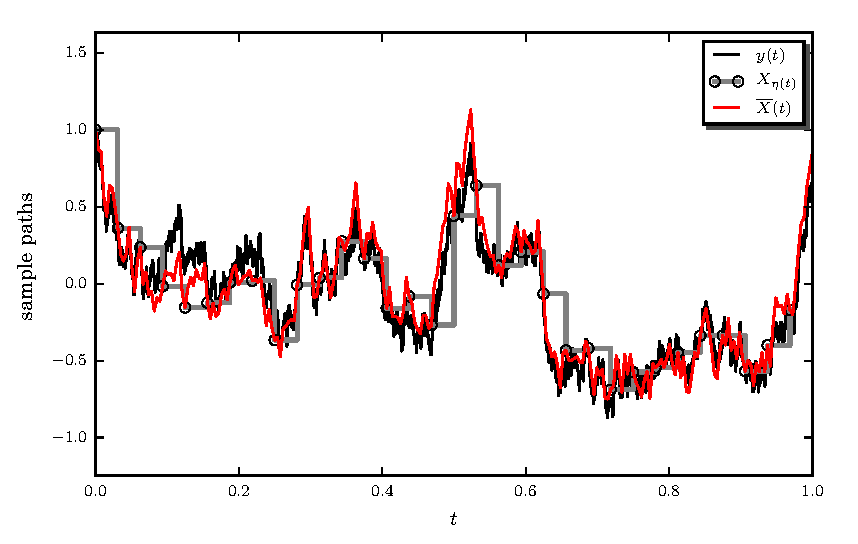
\includegraphics{papers/paperB/sections/ContinuousExtPy/ContinuousExtension.eps}
	\caption{
		The red line represents the continuous extension of the EM scheme. The continuous gray line is the 
		$Y_{\eta(t)}$ 
		process defined in \eqref{eqn:EulerMaruyama} and black line denotes the exact solution of 
		SDE \eqref{eqn:SDE}.
	}
	\label{fig:ContinuousExtension}
\end{figure}
Using the continuous extension \eqref{eqn:EMContinuousExtension}
and the uniform mean square norm, the authors use a stronger version of the ms-error%, which is given by 
$$
	\EX{\sup_{0\leq t \leq t}|y(t)-\overline{Y}(t)|^2}.
$$
%
In  order to prove strong convergence of the EM method, the following assumptions are required.
\begin{assumption}\label{ass:HighamAssumption}
	For each $R>0$ there is a positive constant $C_R$, depending only on $R$, such that
	\begin{equation}\label{ass:LipschitzCondition}
		|f(x)-f(y)|^2 \vee |g(x)-g(y)|^2 \leq C_R|x-y|^2,
		\quad
		\forall x,y\in \R^d 
		\text{ with } |x|\vee |y|\leq R.
	\end{equation}
	And for some $p>2$, there is a constant $A$ such that
	\begin{equation}
		\EX{\sup_{0\leq t\leq T}|\overline{Y}(t)|^p}
		\vee
		\EX{\sup_{0\leq t\leq T}|y(t)|^p} \leq A.
	\end{equation}
\end{assumption}
In \cite{Higham2002b}, the authors prove that the \Cref{ass:HighamAssumption} is sufficient to ensure strong 
convergence for the EM scheme, namely: 
\begin{thm}[
	{\cite[Thm 2.2]{Higham2002b}}
	]\label{thm:HighamMaoStuart}
	Under \Cref{ass:HighamAssumption}, the EM scheme \eqref{eqn:EulerMaruyama} with continuous extension
	\eqref{eqn:EMContinuousExtension}
	%\eqref{eqn:EMIntegralContinuousExtension} 
	satisfies
	\begin{equation}
		\lim_{h\to 0}
		\EX{\sup_{0\leq t\leq T}|\overline{Y}(t)-y(t)|^2}=0.
	\end{equation}
\end{thm}
	
	Applying this result, the strong convergence of an implicit split-step variant of the EM, the
SSEM method is proved . 
Their technique consist in proving each assertion of the following steps.
\begin{enumerate}[\bf{Step} 1:]
	\item
		\label{stp:EMCorrespondence}
		The SSEM for SDE \eqref{eqn:SDE1} is equivalent to the EM for the following conveniently SDE
		\begin{equation}\label{eqn:PerturbedHighamSDE}
			dy_h(t)= f_h(y_h(t))dt +g_h(y_h(t))dW(t).
		\end{equation}
	\item\label{stp:PerturbedSolution}
			The solution of the modified SDE \eqref{eqn:PerturbedHighamSDE} has bounded moments and it is 
			"close" to  $y$ the sense of the uniform mean square norm 
			$
				\EX{\sup_{0\leq t\leq T}|\cdot|^2}
			$.
	\item
	\label{stp:MethodBoundedMoments}
		Show that the SSEM method for the SDE \eqref{eqn:SDE1} has bounded moments.
	\item
		There is a continuous extension of the SSEM, $\overline{Z}(t)$, with bounded moments.
	\item
		Use the above steps and \Cref{thm:HighamMaoStuart} to conclude that
		\begin{equation}
			\lim_{h\to 0}
			\left\{
				\EX{\sup_{0\leq t\leq T}|y_h(t)-y(t)|^2}
			+
			\EX{\sup_{0\leq t\leq T}|\overline{Z}(t) -y_h(t)|^2}
			\right\}=0.
		\end{equation}
\end{enumerate}
In Chapter 4, we will use this technique.
	Moreover, if we are interested in simulating the solution of the SDE \eqref{eqn:SDE} for large periods of time, 
	we need to use stable methods. We can interpret the stability of a numerical scheme, in some sense, as its
	capacity to preserve the  dynamical structure of the solution in that sense. Here we recall the topics that we will 
	work in the next chapter.
\subsection{Numerical Stability}
	With a numerical stability  one obtain  the step sizes for which a method reproduces  behavior of the solution 
	for a SDE. Therefore, it is important to know some qualitative  information  about the  solution, for example: if 
	all solution paths tend to a fixed point, or  if stay on a bounded set or reach an absorbent process.
	Usually the first step in this direction is a linear stability analysis. This study mimics the deterministic 
	context, which is based in the following steps:
	\begin{enumerate}[\bfseries{Step} 1:]
		\item 
			Expand in Taylor series around a fixed point the right hand side of a nonlinear ordinary differential 
			equation $x'(t) = f(t,x)$.
		\item
			Form a linear system with the Jacobian of $f$ evaluated at the equilibrium
			$x'(t) = Ax(t)$.
		\item
			Diagonalize to decouples the linear system and study equations of the form
			$x'(t) = \lambda x(t), \lambda \in \C$.
	\end{enumerate}
	If all eigenvalues of $A$ are different of zero, then the  theorem of Hartman justify the use of this last equation 
	for study behavior around sufficient small neighborhood. So, ones 
	seek conditions for assure that the numerical methods preserves the dynamics of underlying test. 
		
		In stochastic numerics, the history runs similar. But here, the usual test is a linear SDE with 
	multiplicative noise. The advantage of this model is that has the same unique fixed point as its deterministic 
	analogous, the origin \cite[]{Higham2000} . The other test equation is the linear SDE with additive noise. However, 
	for these model the 
	concepts of numerical stability was unclear. The first works with this test 
	\cite{Hernandez1992,Milstein2004,Artemiev1997}, differs about the meaning of fixed point and stability. Recently, 
	the works of \citeauthor*{CruzCancino2010}
	\cite{CruzCancino2010} and \citeauthor*{Buckwar2011a} \cite{Buckwar2011a} analyze these model using the theory of
	random dynamical systems, which in our opinion clarifies this issue.
	
		Naturally the nonlinear case, is even more complex. Although  Lyapunov theory is the usual approach in 
	applications \cite{Khasminskii2011}, a more general novel approach based on the theory of random dynamical 
	systems \cite{Arnold1998} attracts the now days attention. In the following we provide this notions. 
		
\section*{Linear Stability}
	\subsection*{Multiplicative noise}
		Consider the scalar linear SDE
		\begin{equation}\label{eqn:SDEMultiplicativeNoise}
			dy(t)=\lambda y(t)dt+\xi y(t) dW(t) , \quad X_0=x_0,  \quad \lambda,\xi \in \C.
		\end{equation}
		The solutions of this SDE have the following property
		\begin{equation}\label{eqn:LinearMSEquivalence}
			\lim_{t\to\infty} \EX{|y(t)|^2} = 0 \Leftrightarrow \Re(\lambda) +\frac{1}{2} |\xi|^ 2 <0.
		\end{equation}
		A solution that satisfies  the previous limit  is a \emph{mean-square stable} solution. 
		Note that for $\xi = 0$ we have, $\Re(\lambda)<0$, which is the stability condition  for the deterministic case.
			
			Applying the EM method \eqref{eqn:EulerMaruyama} to test \eqref{eqn:SDEMultiplicativeNoise}, we obtain
		\begin{equation}\label{eqn:MS-EMRecurrence}
			Y_{k+1} = \left(1 + h\lambda + \sqrt{h}\xi V_k\right)Y_k,
		\end{equation}
		where each $V_k$ is an independent $\calN(0,1)$ random variable. 
		In order to study the stability properties of the EM, we must therefore study
		the long time behavior of random variables of the form \eqref{eqn:MS-EMRecurrence}.
		Analogously, we will say that sequence \eqref{eqn:MS-EMRecurrence} is mean-square stable if 
		$
			\lim_{k \to  \infty}
				\EX{|Y_k|^2} = 0.
		$
		Note that the EM depends upon the problem parameters $\lambda$ and  $\xi$, and the method
		parameter $h$. Then for a particular choice of parameters, we will say that the EM is mean-square stable 
		if it produces a mean-square stable sequence. 
		Our interest lies in finding the parameter values for which the EM method is stable, and comparing results
		with the region $\Re(\lambda) + \frac{1}{2}|\xi|^2 < 0$ in \eqref{eqn:LinearMSEquivalence}
		for the underlying SDE (see \Cref{fig:StabilityPlotsMultiplicativeEM}). In this line we have the following 
		result. 
		\begin{thm}
			Consider the EM method for the linear scalar SDE \eqref{eqn:SDEMultiplicativeNoise}. If the parameters 
			$\lambda$, $\xi$, and the step size $h$ satisfies
			$$
				\Re(\lambda) + \frac{1}{2}
				\left( |\xi|^2 + h|\lambda|^2\right) <0.
			$$
			Then the EM solution is \emph{mean square stable}.
		\end{thm}
		
		\begin{figure}[htb]
			\centering
			\includegraphics[scale=0.6]{Preliminaries/figures/StabilityPlotsMultiplicativeEM.png}
			\caption{Mean square regions of stability. The horizontal lines represents the stability region of
				SDE \eqref{eqn:SDEMultiplicativeNoise} and diagonal lines for the EM solution.
			}
			\label{fig:StabilityPlotsMultiplicativeEM}
		\end{figure}
			
	\subsection*{Additive noise}
	Here we study the additive linear SDE: 
	\begin{equation}\label{eqn:SDELinearAdditive}
		dy(t)=\lambda y(t)dt+ \xi  dW(t) , \qquad y_0=y_(t_0), \qquad \lambda, \xi \in \R.		
	\end{equation}
	where $\lambda$, $\xi \in \mathbb{C}$ and $X_{t_0}$ is the initial value of the process
	at time $t_0$. Equation \eqref{eqn:SDELinearAdditive}  has  the following  exact solution:
	\begin{equation}\label{eqn:OUProcess}
	y(t)=\exp(\lambda (t-t_0)) y(t_0)+\xi 
	\exp(\lambda t)\int\limits_{t_0}^{t}\exp(-\lambda s)dW(s), 
	\qquad t\geq t_0.
	\end{equation}
	The stochastic process $y(t)$ defined in \eqref{eqn:OUProcess} is known as 
	the {\it Ornstein-Uhlenbeck}'s (OU)  process. According to \cite{Hernandez1992},
	the OU process  is {\it asymptotically mean stable} if
	$ \lim_{t\to\infty}\m{y(t)}=0$ and is
	{\it  asymptotically  mean square stable} if
	$\displaystyle \lim_{t\to\infty}\ms{y(t)}=-\xi/2Re(\lambda)$. Both 
	limits are verified if $\lambda<0$. 
	Analogous stability properties are given for 
	stochastic  difference equations with additive noise \cite{SaiotoPreprint}. 
	Now, if we consider $\lambda<0$ then the OU solution \eqref{eqn:OUProcess} does 
	not convergence as $t$ tends to infinity but has the following pullback limit:
	\begin{equation}\label{eq4}
		\lim_{t_0\to-\infty} y(t)=\widehat{O}_t:=
		\exp(\lambda t)\int\limits_{-\infty}^{t}\exp(-\lambda s)dW(s), 
	\end{equation}
	$W(t)$  is now defined for all $t\in\mathbb{R}$, see
	\cite{Arnold1998, kloeden1999towards}. Furthermore, the process \eqref{eq4} is a
	stationary solution  of the additive linear SDE which attracts all other solutions in
	forward time and path-wise sense. Moreover, it is a finite process for all $t\geq
	T_{D(\omega)}$ ($\omega\in \Omega$) for  appropriate families $D(\omega)$ of bounded
	sets of initial conditions, see \cite{Robinson2002}. Therefore, 
	we can evaluate the numerical stability of a given stochastic method by examine if 
	this scheme reproduce the pullback asymptotic behavior.
	For example, the explicit EM scheme for \eqref{eqn:SDELinearAdditive}
	$$
		Y_{k+1} = (1+\lambda h) Y_n + \xi \Delta W_n,	
	$$
	given a initial value $Y_{k_0}$, has the form
	$$
		Y_{k+1} = (1+\lambda h)^{k-k_0} Y_{k_0}
			+\xi \sum_{j=k_0}^{k-1} (1+\lambda h)^{k-1-j} \Delta W_j.
	$$
	So, the path-wise pullback limit (taking $k_0 \to \infty$  with $k$ held fixed and $Y_{k_0} = Y_0$ for
	all $Y_{k_0}$ and constant time step $h$) exists, provided that $0 <h< 2/(- \lambda)$, $\lambda <0$, and is given
	by
	$$
		\widehat{O}_k^{(h)} := 
			\xi \sum_{j= -\infty}^k
				(1+\lambda h)^{1-k-j} \Delta W_j,
	$$
	for more details see the work of
	\citet*{Buckwar2011a}.
	
\section*{Non-Linear Stabbility}	
	Now we discuss the nonlinear case for multiplicative and additive noise. 
	\subsection*{Multiplicative Noise}
	We start with a notion of stability	which emulates the continuity respect to initial conditions of deterministic 
	ODEs.
	\begin{dfn}[\citeauthor{Baker2000a} {\cite{Baker2000a}}]\label{dfn:SNMS}
		Let $Y_n$ and $\widehat{Y}_n$ two different numerical recurrences  with
		corresponding initial process  $Y_0$ and $\widehat{Y}_0$. We shall say that a
		discrete time, $Y$ is \emph{numerically zero-stable in quadratic mean-square sense} if given
		$\epsilon >0$, there  are positive constants $h_0$ and $\delta=\delta(\epsilon,h_0)$
		such that for all $h\in(0,h_0)$ and positive integers $n \leq T/h$ whenever
		$\ms{Y_0-\widehat{Y}_0}<\delta$ then
		\begin {eqnarray}\label{eqn:SNMS}
		\rho_n :=
		\ms{Y_n-\widehat{Y}_{n}}<\epsilon .
	\end{eqnarray}
	If the method is stable and $\rho_n \to 0$ when $n\to \infty$, then the method is
	\emph{asymptotically zero-stable in the quadratic mean-square sense}.
\end{dfn}
Also, in \cite{Baker2000a} provides a result to characterizes this type of stability. Here we
enunciated it for the EM.
\begin{thm}[{\cite[Thm. 4 ]{Baker2000a}}]
	Let $C_1$, $C_2$ and $C_3$ generic positive constants which not depends on $h$ and $V$ a
	$\calN(0,1)$ random variable. 
	If the coefficients of  SDE \eqref{eqn:SDE} satisfies the estimates
	\begin{align*}
		\left|\EX{
			f(x) h +  g(x)\sqrt{h}V -
			\left(
				f(x') h + g(x')\sqrt{h}V
			\right)}	
		\right| 
		&\leq C_1h \left(|x - x'| \right), \\
		\EX{\left|
				hf(x)+g(x)\sqrt{h}V -
				\left(
				 f(x') h + g(x')\sqrt{h}V
				\right)	
			\right|^2}
			&\leq C_2 h \left(|x - x'| \right),
	\end{align*}
	then the EM method \eqref{eqn:EulerMaruyama} for \eqref{eqn:SDE} is zero-stable in the quadratic mean-square sense.
\end{thm}
%%%%%%%%%%%%%%%%%%%%%%%%%%%%%%%%%%%%%%%%%%%%%%%%%%%%%%%%%%%%%%%%%%%%%%%%%%%%%%%%%%%%%%%%%%
\subsection*{Additive noise}
		Nonlinear differential equations have more complex  dynamics than the linear case and
	the same  occurs for the finite difference equations. So,  \citeauthor*{Caraballo2006} in
	\cite{Caraballo2006}  extend the nonlinear stability theory of the deterministic
	numerical  analysis given in \cite{kloeden1999towards} to the stochastic
	case. They propose and justify the use of the following SDE as a test equation with additive noise:
	\begin{equation}\label{eqn:SemilinearSDE}
		dy(t)=\left(Ay(y)+f(y(t))\right)dt+\xi dW(t),
	\end{equation}
	where $A$ is a $d \times d$ stiff matrix and function $f : \R^d \to \R^d $ is a nonlinear and non-stiff function 
	that satisfies, a
	{\it contractive one-sided Lipschitz} condition with constant
	$L_1>0$
	\begin{equation}\label{cl}
		\langle
			u - v,f(u)-f(v)
		\rangle\leq
		-L_1|u-v|^2\qquad \forall u,v\in \mathbb{R}^d.
	\end{equation}
Also the authors give sufficient conditions to assure an asymptotically stable stochastic stationary solution
of \eqref{eqn:SemilinearSDE}. In this context establish the following result for the stability of $\theta$-EM scheme.
\begin{thm}[{\cite[Thm. 3.1]{Buckwar2011a}}]
	Suppose that the drift coefficient satisfies a contractive one-sided Lipschitz condition, and that the vector field 
	f satisfies a globally Lipschitz condition . Then the $\theta$-EM scheme has a unique stochastic stationary 
	solution 
	which is pathwise asymptotically stable for all step sizes $h> 0$
	if
	$$
		(1-\theta) (|A|+L) <-\theta (\mu[A] - L_1),
		\qquad
		\mu[A] = \lim_{\delta \to 0^+} \frac{(|Id + \delta A|)}{\delta},
	$$
	where $L$ refers to the Lipschitz condition and $L_1$  the to contractive one-sided Lipschitz condition.
\end{thm}












The following chapter shows adaptations of these results for the construction of a new method, the Steklov method.

